\section{First Order Roe Scheme with Flat Bottom}
\subsection{Scheme}
We first implement the first order Roe scheme to simulate the shallow water equations for a flat bottom. The algorithm works as follows. We have our equation set up as a conservation law i.e.,
$$q_t+f(q)_x=0$$
so we need a method in conservation form, i.e.
$$Q_i^{n+1} = Q_i^n - \frac{\Delta t}{\Delta x}(F^n_{i+1/2}-F^n_{i-1/2})$$ 
We use the following numerical flux formula
$$F_{i+1/2}=\frac{1}{2}(f(Q_i^n)+f(Q_{i+1}^n))-\frac{1}{2}\sum_{p=1}^2 \lvert \hat{\lambda}_{j+1/2}^p \rvert W_{j+1/2}^p$$
From the previous section, we have 
$$f(q) = \begin{pmatrix}
q_2\\ \frac{q_2^2}{q_1} + \frac{gq_1^2}{2}
\end{pmatrix}$$
From the course text book we have $\hat{\lambda}^1_{j+1/2} = \hat{u}-\hat{c}$ and $\hat{\lambda}^2_{j+1/2} = \hat{u}+\hat{c}$ where $\hat{c}=\sqrt{0.5g(h_{i-1}+h_i)}$,
$$\hat{u}=\frac{\sqrt{h_{i-1}}u_{i-1}+\sqrt{h_i}u_i}{\sqrt{h_{i-1}}+\sqrt{h_i}}$$ 
and letting $\delta = Q_i - Q_{i-1}$ we get $W^1_{i-1/2}=\frac{(\hat{u}+\hat{c})\delta^1 - \delta^2}{2\hat{c}}\begin{pmatrix}
1\\ \hat{u} - \hat{c}
\end{pmatrix}$ and $W^2_{i-1/2}=\frac{-(\hat{u}-\hat{c})\delta^1 + \delta^2}{2\hat{c}}\begin{pmatrix}
1\\ \hat{u} + \hat{c}
\end{pmatrix}$.

\subsection{Single pulse}
We are now going to use this scheme a produce a single pulse, with "wall" boundary condition. We were given the following initial condition for the height :
$$h(x,0) = H + ae^{-(x-L/2)^2/w^2}$$

With $H =1$, $w=0.1L$ and $a=H/5$. The goal is now to find $m(x,0)$ so that we only have one wave traveling. To find this initial condition, let us diagonalize the PDE using the chain rule. Because we have a flat bottom ($B_x=0$), the chain rule gives :
$$q_t+(f(q))_x = q_t + f'(q)q_x = \left(\begin{array}{c}
q_1 \\ 
q_2
\end{array}\right)_t + 
\left(\begin{array}{cc}
0 & 1 \\ 
-\frac{q_2^2}{q_1^2}+gq_1 & 2 \frac{q_2}{q_1}
\end{array}\right)\left(\begin{array}{c}
q_1 \\ 
q_2
\end{array}\right)_x = \left(\begin{array}{c}
0 \\ 
0
\end{array}\right)  $$ 

To diagonalize this system, we will need the eigenvalues of $f'(q)$. Let us compute them :
$$det(\lambda I - f('q))= det(\left(\begin{array}{cc}
\lambda & -1 \\ 
\frac{q_2^2}{q_1^2}-gq_1 & \lambda - 2 \frac{q_2}{q_1}
\end{array}\right)) = \lambda^2 - 2\frac{q_2}{q_1}\lambda + \frac{q_2^2}{q_1^2}-gq_1 = 0$$

Solving this equation gives us the two eigenvalues : 
$$\lambda_1 = \frac{q_2}{q_1} + \sqrt{gq_1}$$
$$\lambda_2 = \frac{q_2}{q_1} - \sqrt{gq_1}$$

Looking at first line of $\lambda I -f'(q)$, it is easy to see that the eigenvectors are given by : 
$$p_1 = \left(\begin{array}{c}
1 \\ 
\lambda_1
\end{array}\right)$$
$$p_2 = \left(\begin{array}{c}
1 \\ 
\lambda_2
\end{array}\right)$$

Let us define $P(q) = [p_1\: p_2]$. So the system becomes :
$$q_t + P(q)\Lambda(q) P(q)^{-1} q_x = 0$$
$$P(q)^{-1}q_t + \Lambda(q) P(q)^{-1} q_x = 0$$

Let us now make the assumption that $P(q)$ is constant and so $P(q)=P$. Then, we can define $w=P^{-1}q$ so that :
$$w_t + \Lambda w_x = 0$$

To have a single pulse, we would then need to have one eigenvalue equal to 0. In our case, let us pick $\lambda_2 =0$ : 
$$\lambda_2 = 0 \iff q_2 = q_1\sqrt{gq_1}$$

This relation could be used to compute $m(x,0)$ : 
$$m(x,0) = h(x,0)\sqrt{gh(x,0)}$$

However, in practice, that does not work. In spite of that, we can think of an initial condition that is similar to that one and give good results. We chose :
$$m(x,0) = (h(x,0) - H)\sqrt{gh(x,0)}$$

\begin{figure}
\begin{center}
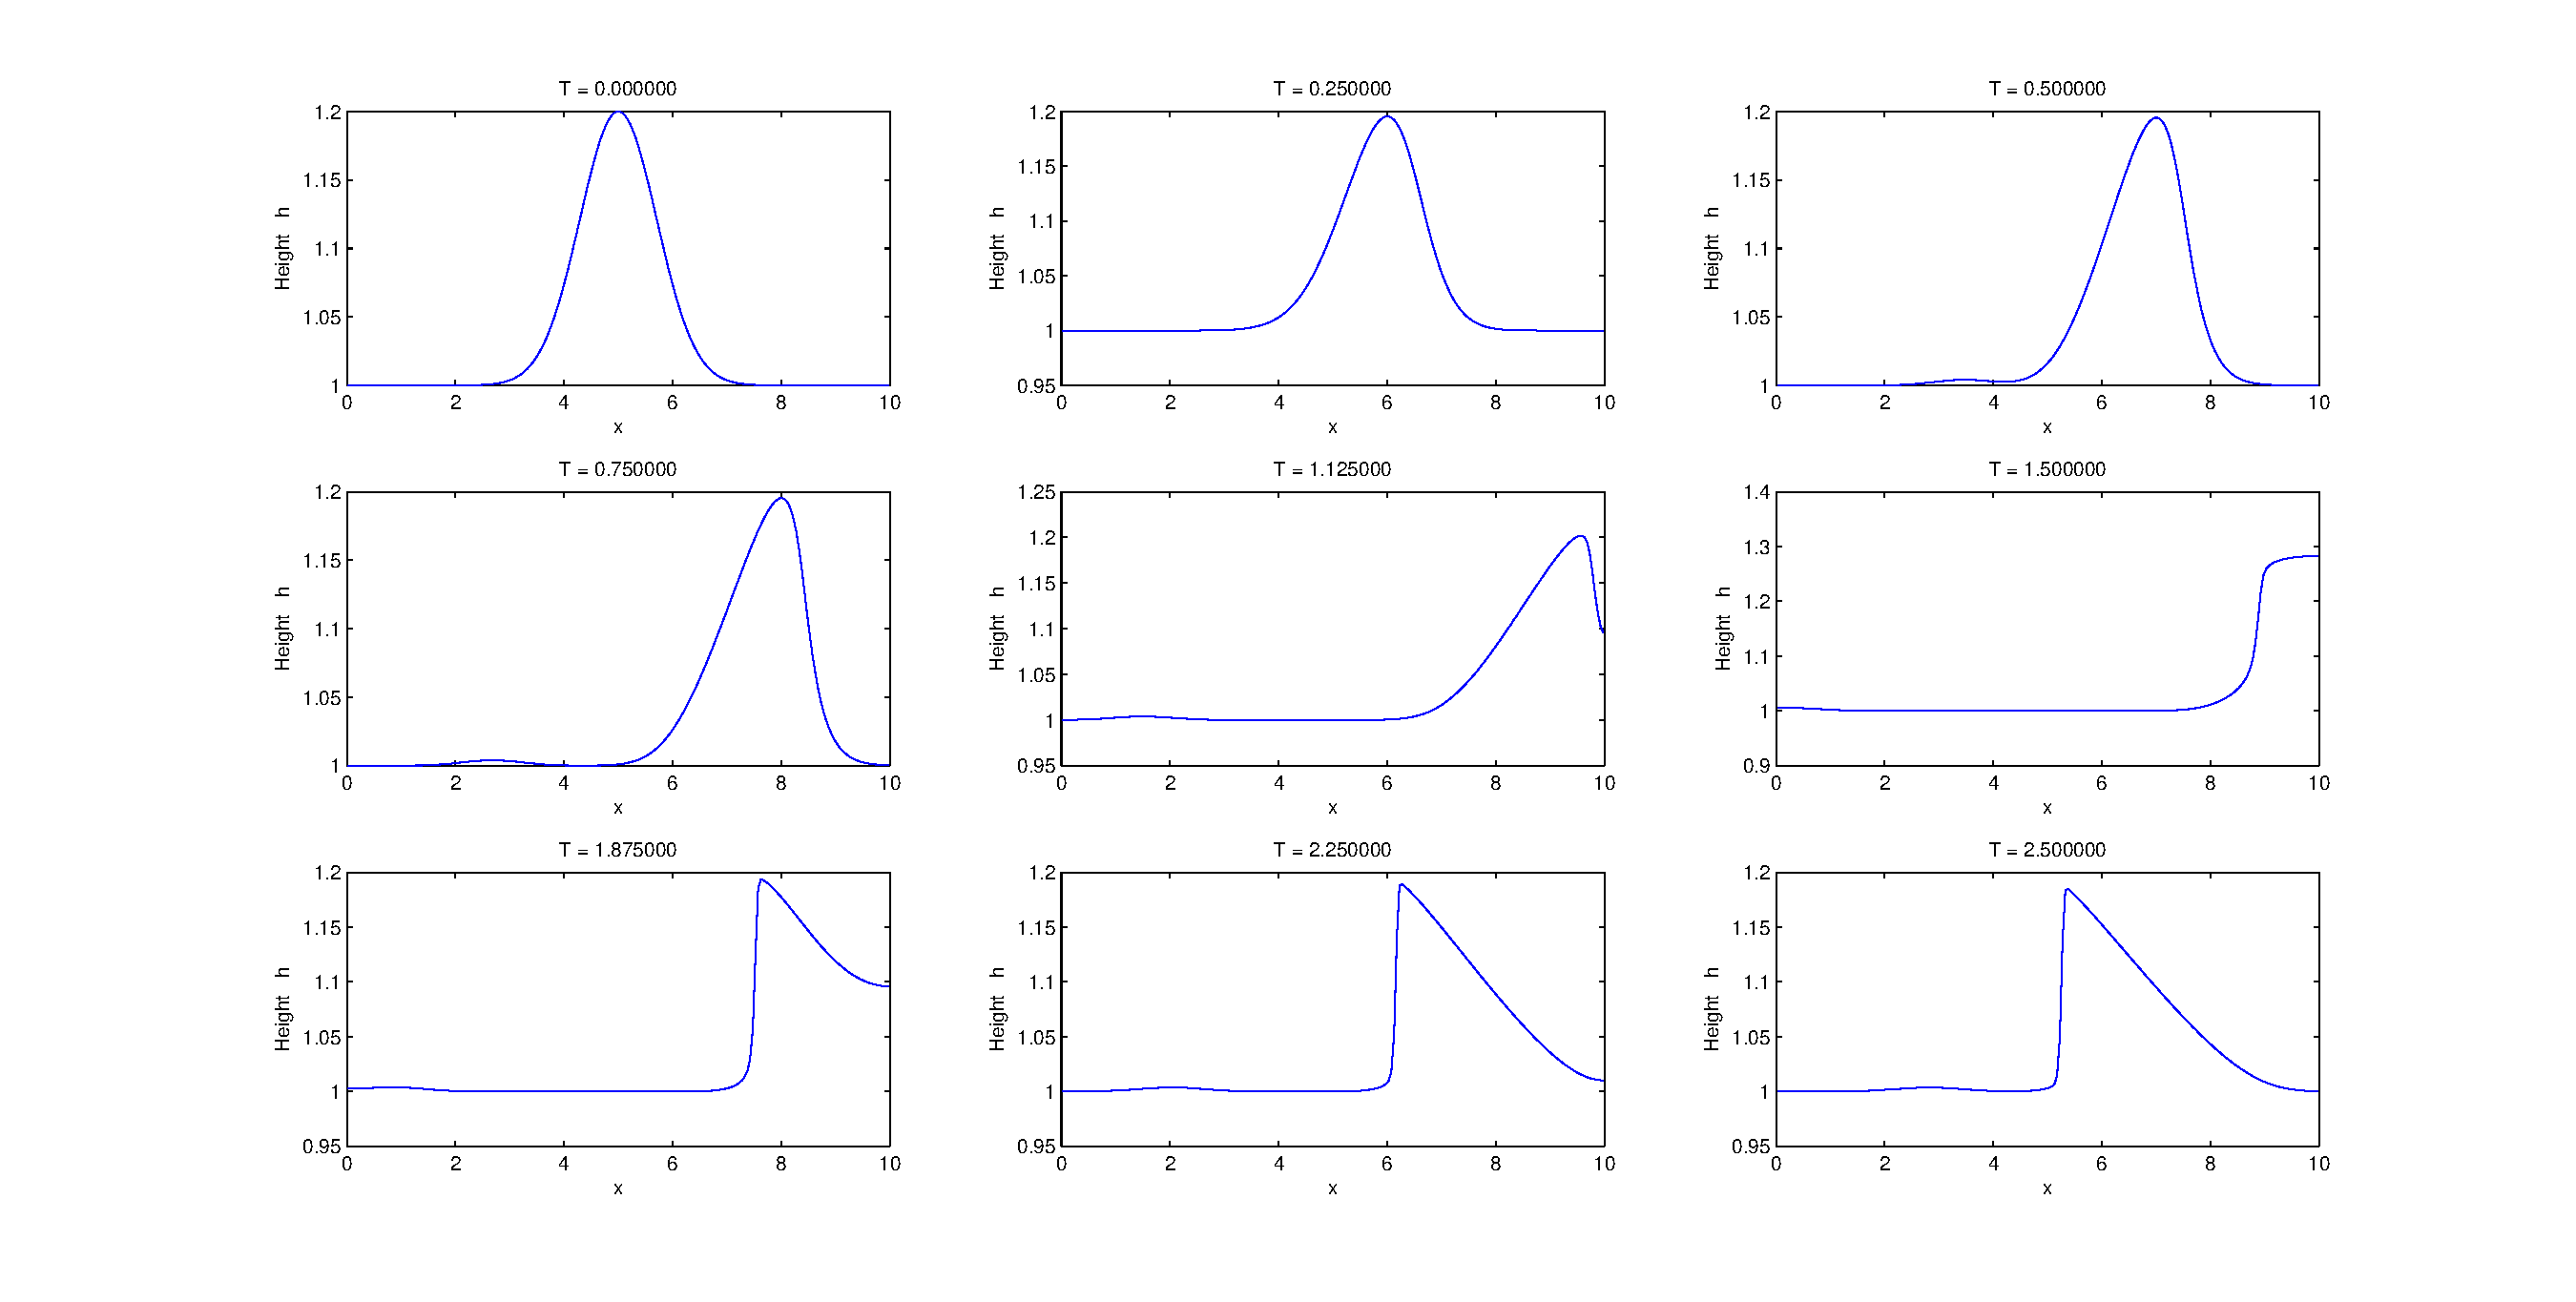
\includegraphics[scale=0.35]{firstTry.eps}
\caption{$m(x,0) =(h(x,0) - H)\sqrt{gh(x,0)}$ }
\label{firstTry}
\end{center}
\end{figure}

Figure \ref{firstTry} gives the evolution of the pulse for different times. We can see that it is good but not perfect. We mostly see one pulse going to the right then bouncing off the wall but we also see a really small pulse going to the left. This pulse is most visible at $T=0.5$.

To come around this imperfection, we tried to change $m(x,0)$ by multiplying it by a constant. We found the best result with a factor of 1.05.

\begin{figure}
\begin{center}
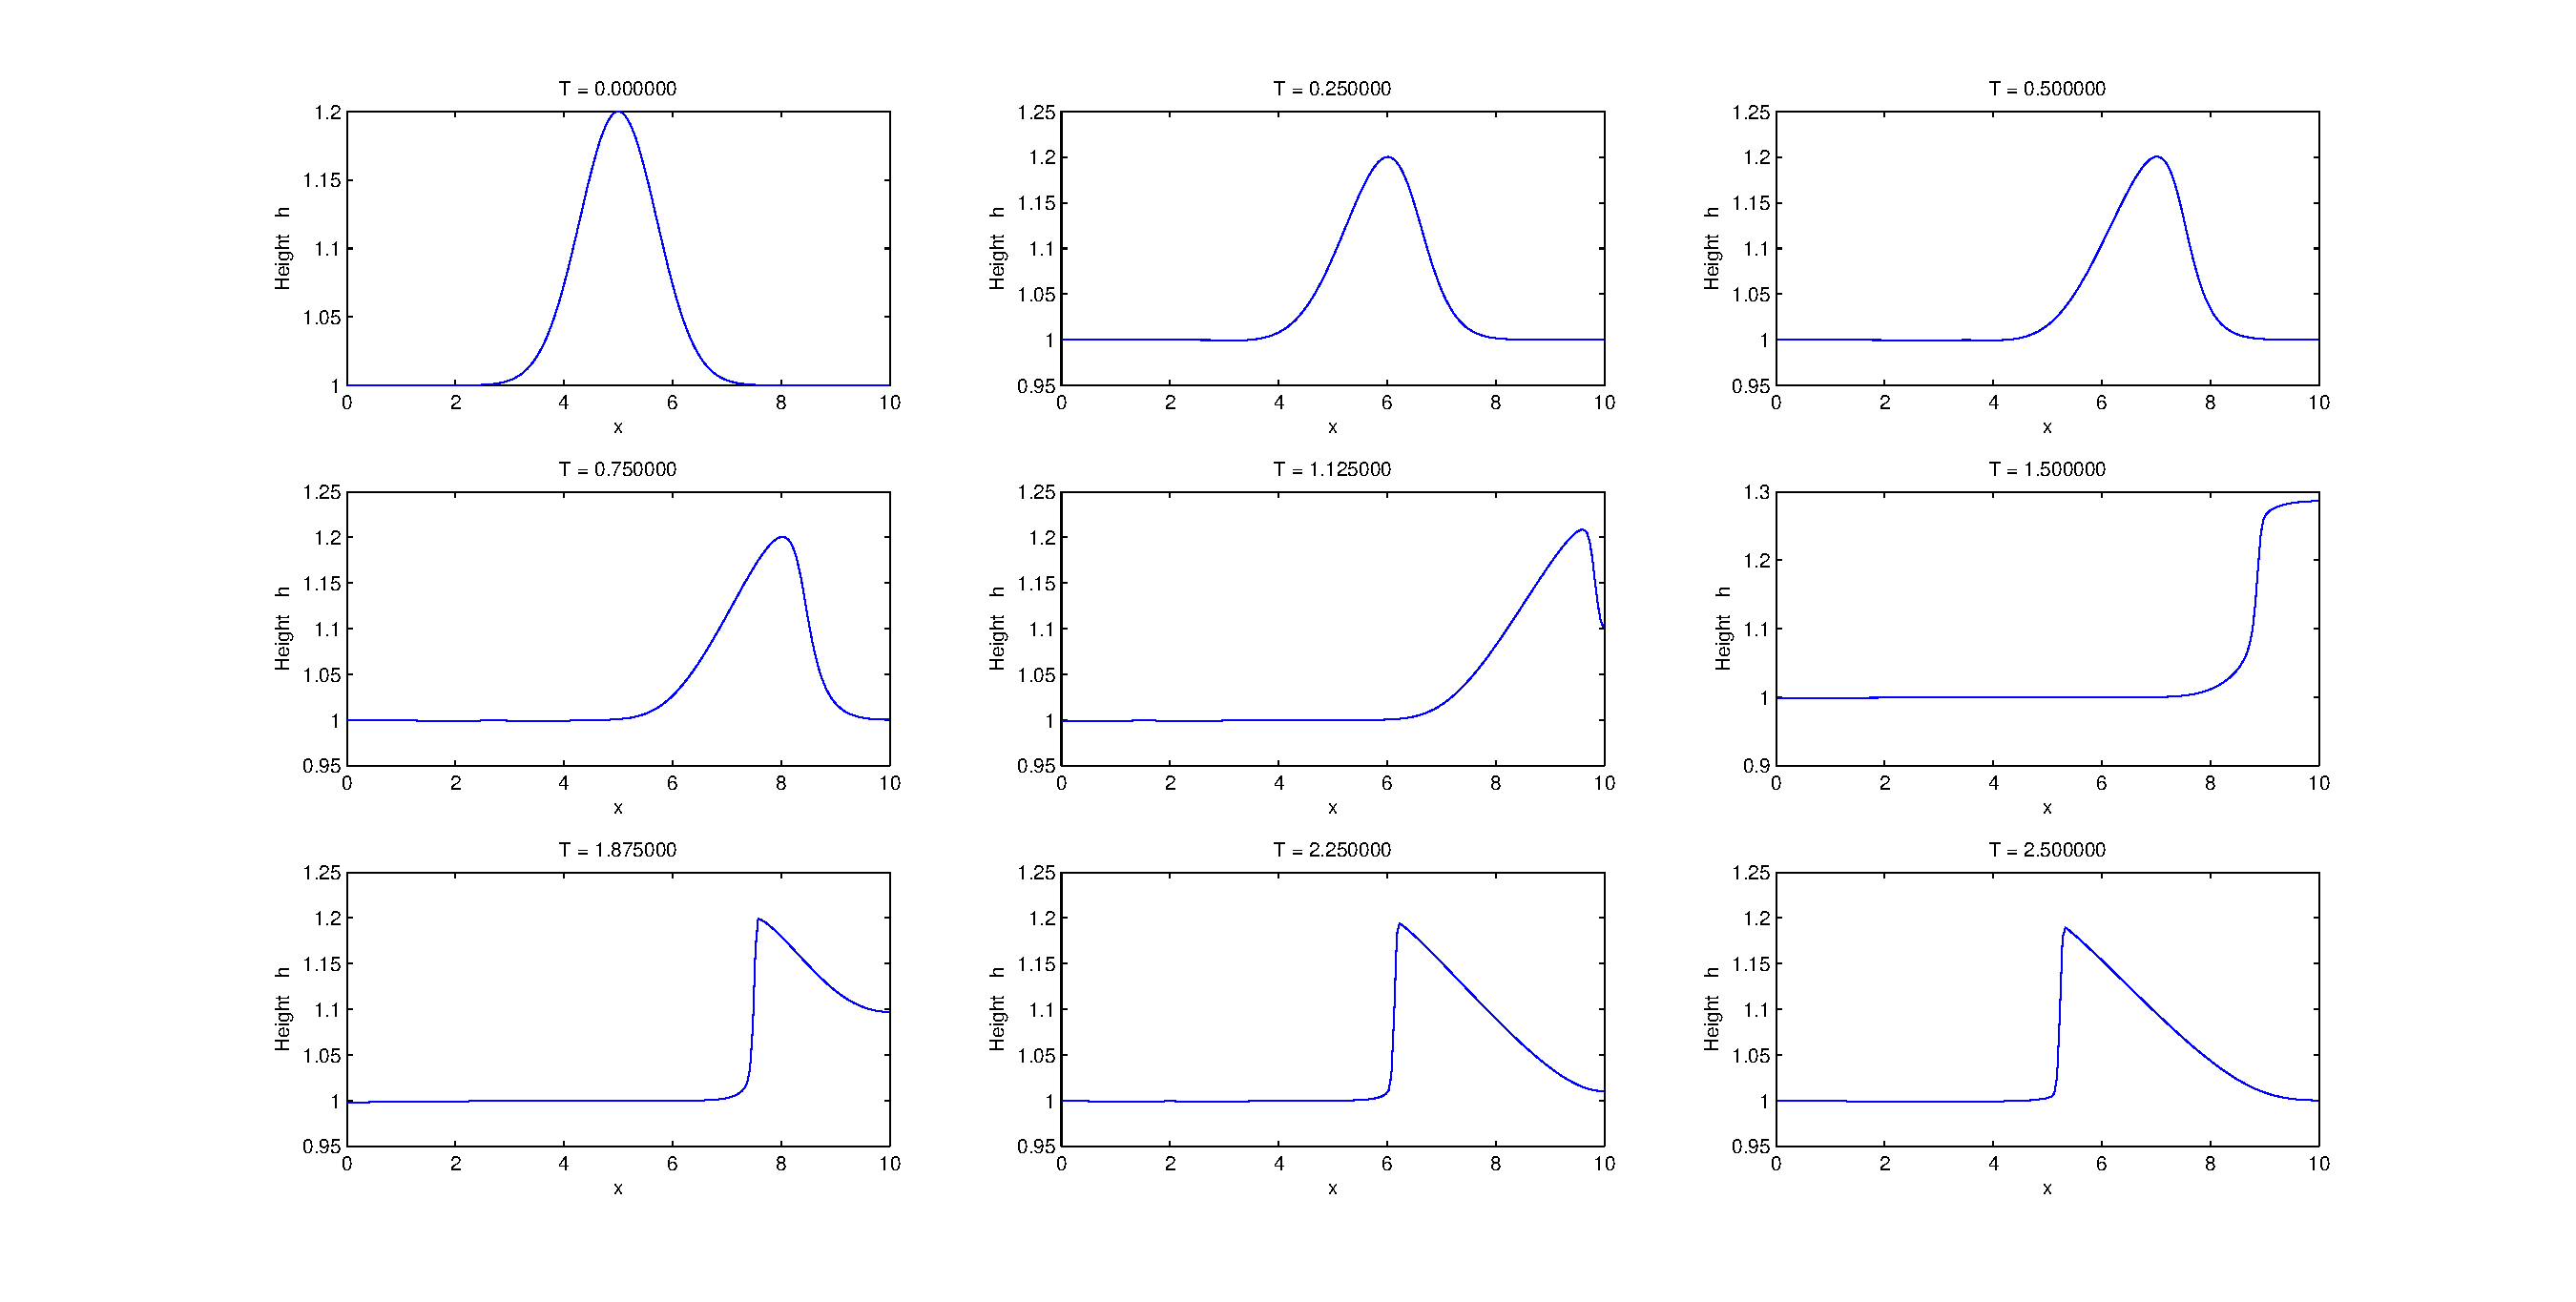
\includegraphics[scale=0.35]{secondTry.eps}
\caption{$m(x,0) =1.05(h(x,0) - H)\sqrt{gh(x,0)}$ }
\label{secondTry}
\end{center}
\end{figure}

Figure \ref{secondTry} shows the results when a factor of 1.05 is applied. We can see that it is much better and we do not see the small pulse.

\subsection{Results with the Roe solver}
We are now going to run the Roe solver with different number of grid points and compare the results. We can first note that, in order to have stability, the ratio of space and time steps must be such that : 
$$\frac{\Delta t}{\Delta x} \leq 0.25$$

We will always use the ratio as high as possible so $\frac{\Delta t}{\Delta x}=0.25$. 
\begin{figure}
\begin{center}
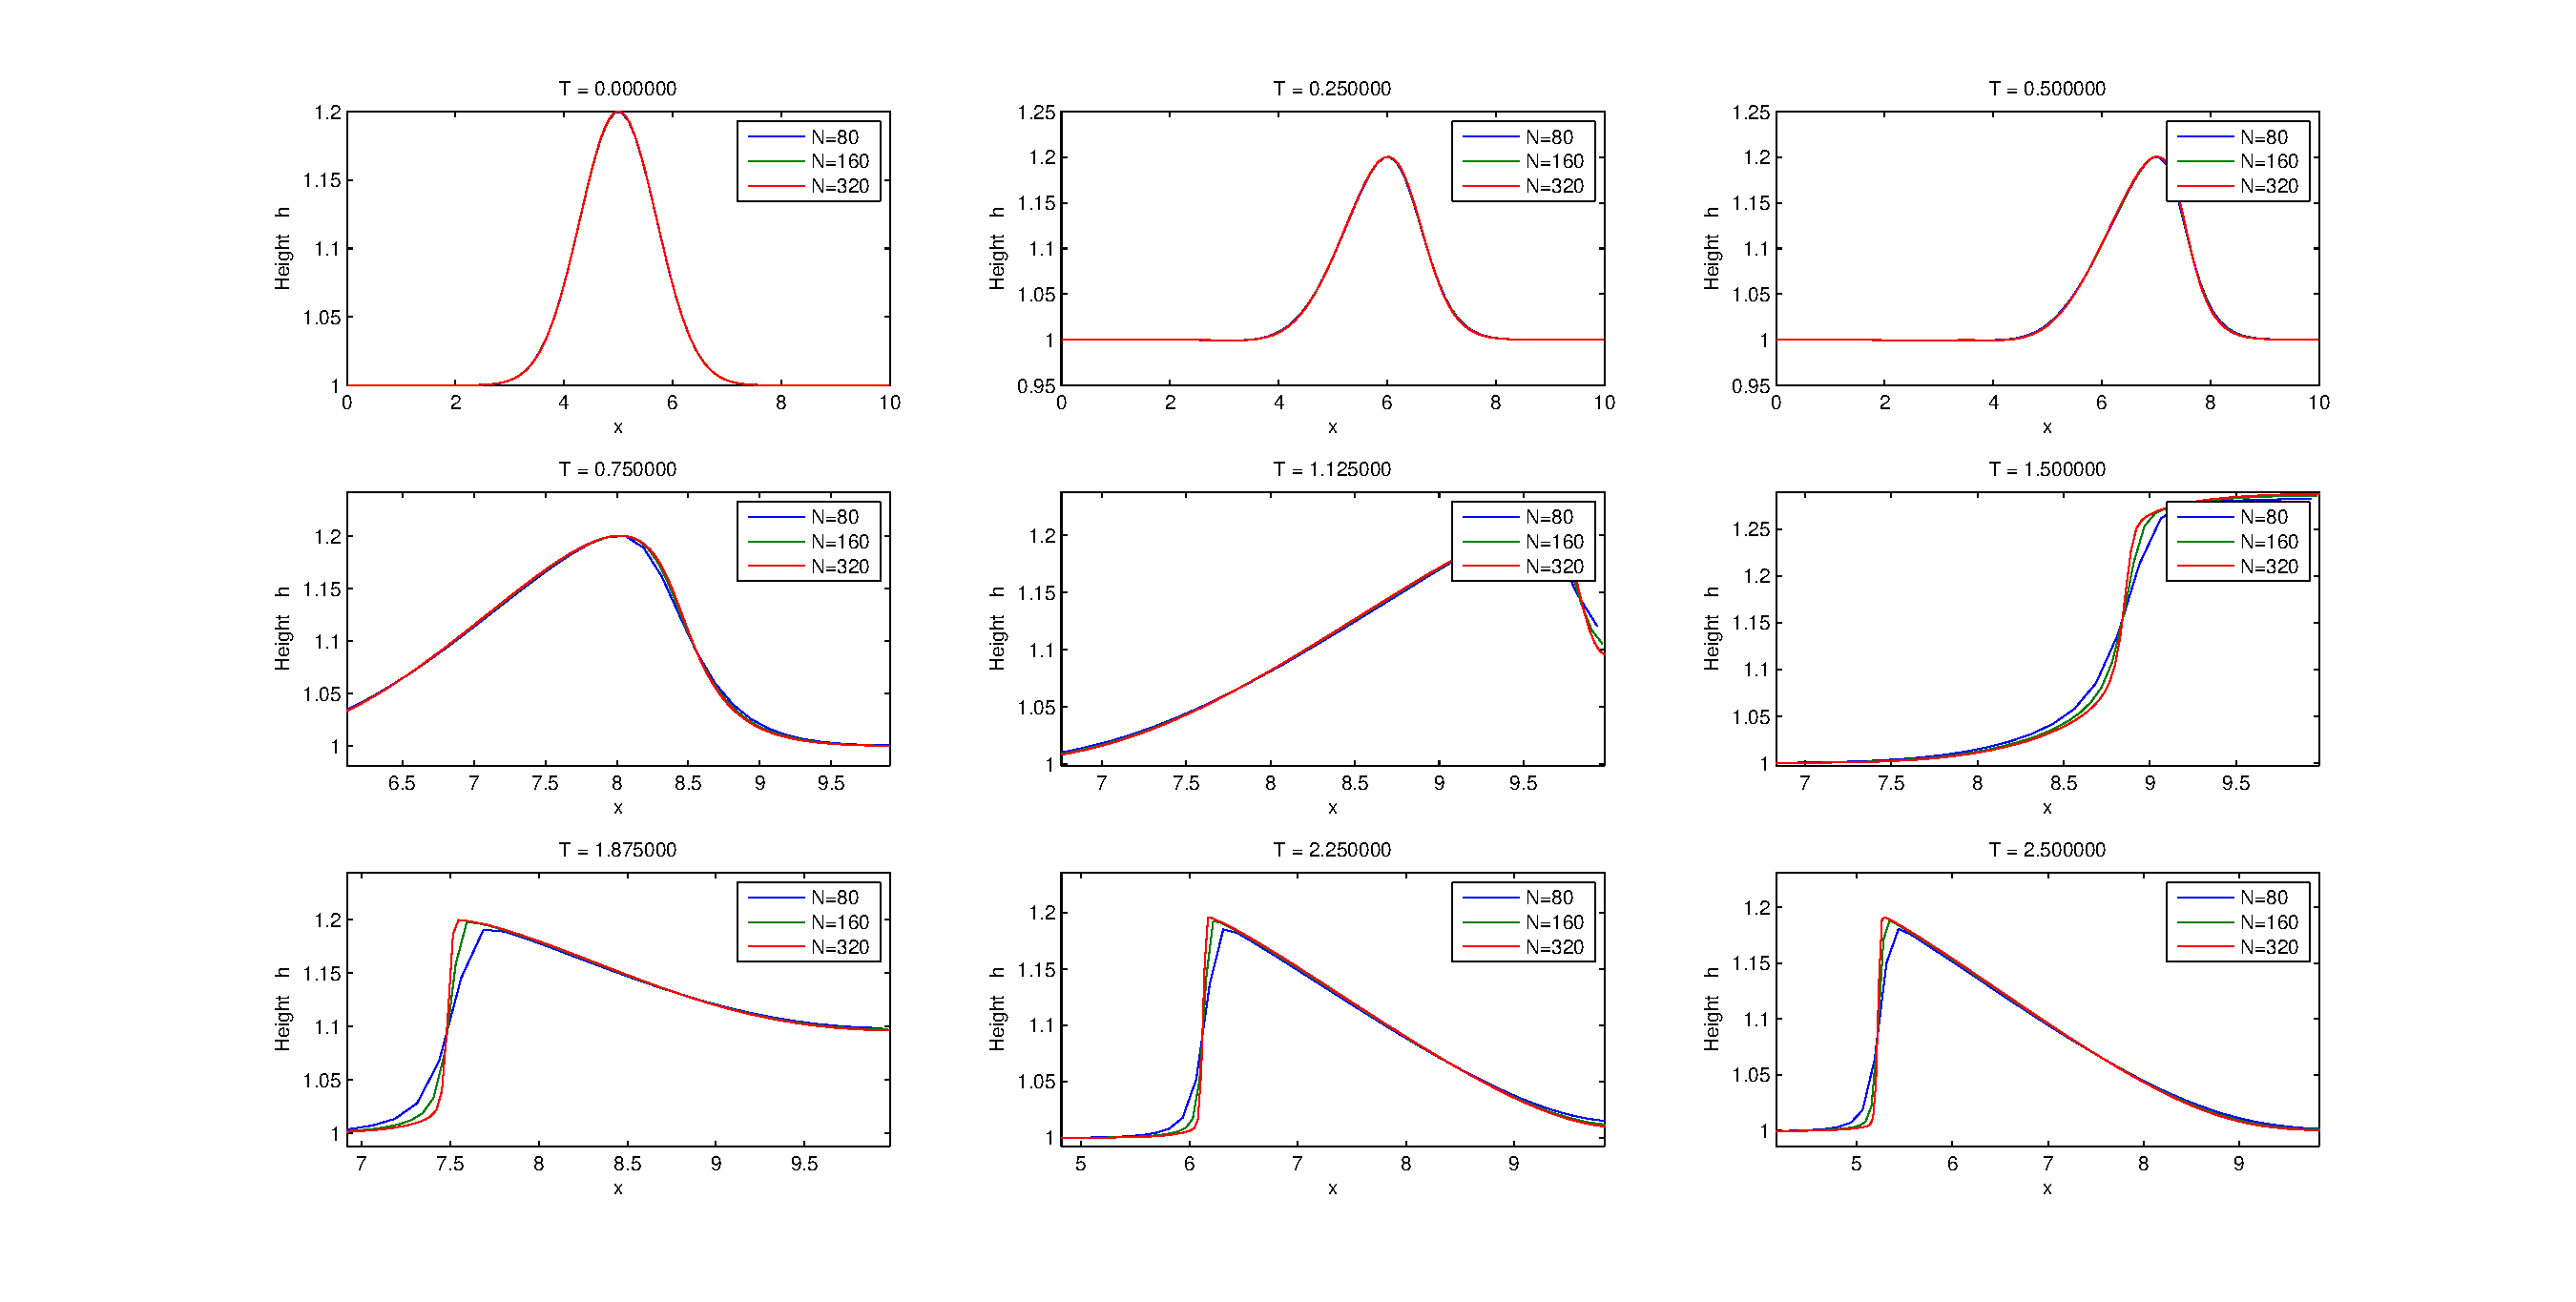
\includegraphics[scale=0.35]{comp.eps}
\caption{Comparison of the solution for $N=80,160,320$}
\label{comp}
\end{center}
\end{figure}

Figure \ref{comp} shows the results. Some subfigures are zoomed in so that the reader can see the difference more easily. We can see that before the wave touch the boudnary, all solutions are essentially the same. But as the edge of the wave become sharper, the finer grid gives better results. For the coarser discretization, the edge is smoother and the peak not as high. There is thus more dissipation when the grid is coarse.

\subsection{Comparison with Lax-Friedrichs}
Let us now compare the solution obtained with Roe scheme with the one computed in homework 2 with Lax-Friendrichs scheme. The comparison was done with $N=320$ and the initial conditions given earlier in the report, for both Roe scheme and Lax-Friedrichs scheme.

\begin{figure}
\begin{center}
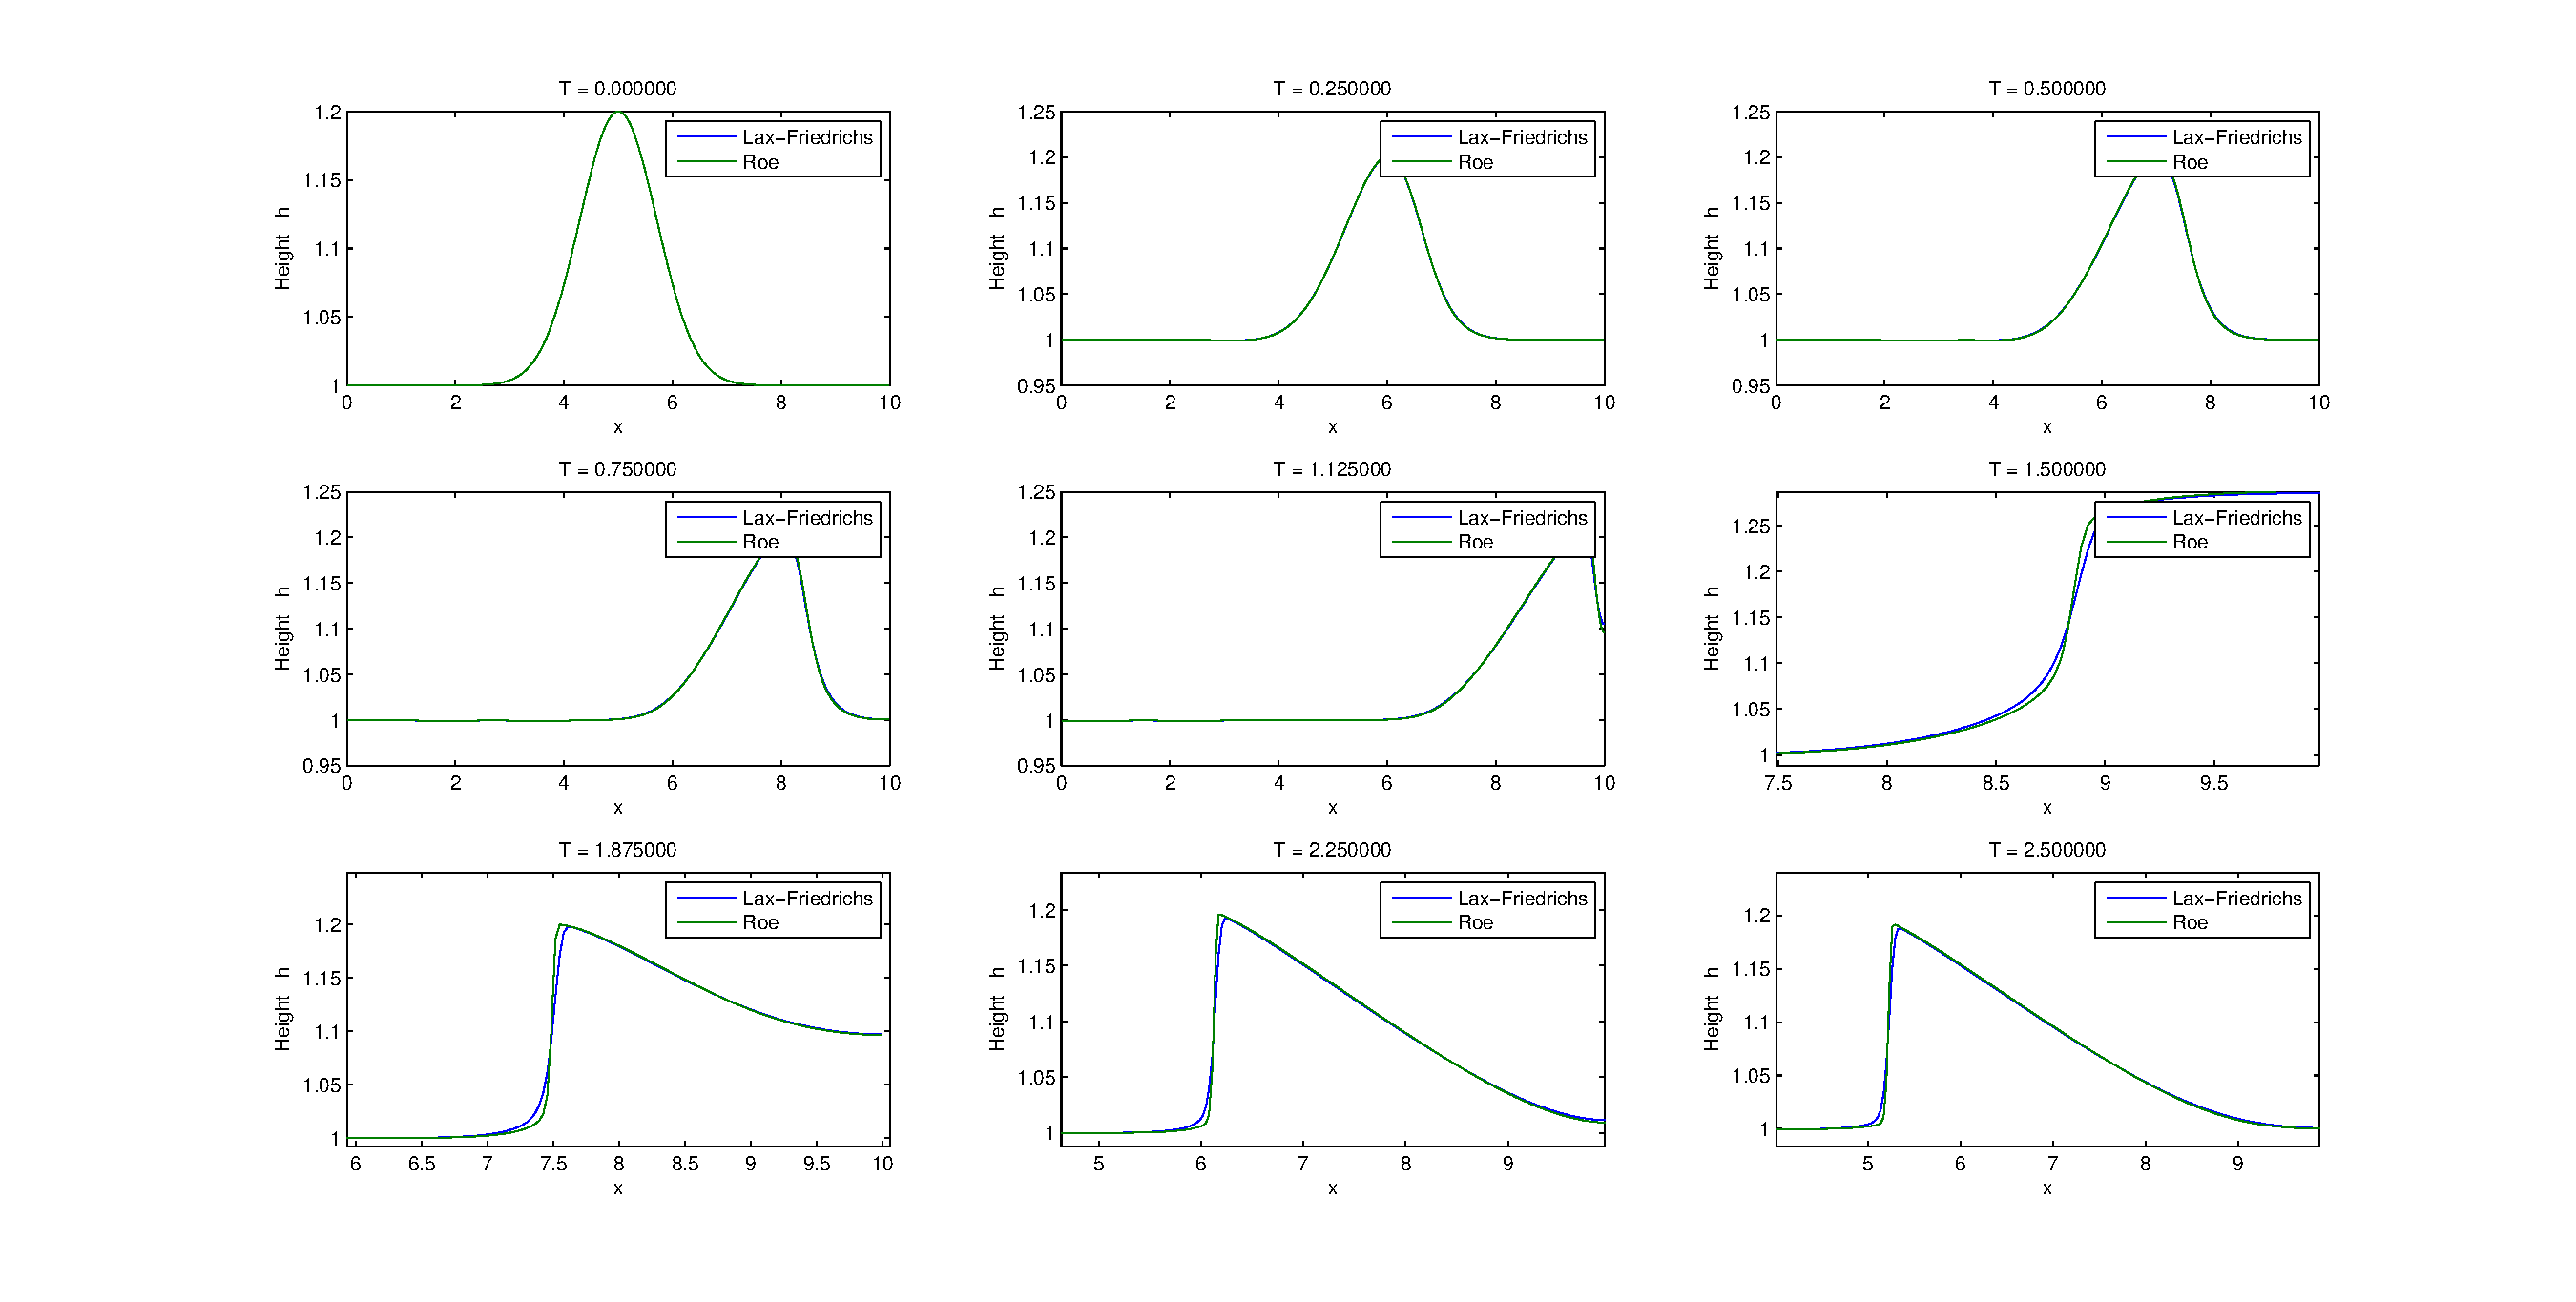
\includegraphics[scale=0.35]{roeComp.eps}
\caption{Comparison of Roe with Lax-Friedrichs for $N=320$}
\label{roeComp}
\end{center}
\end{figure}

Figure \ref{roeComp} gives the results. Once again, some parts have been zoomed in. We can seen that before the wall, the two solutions are on top of each other. After the wall tough, when the edge of the wave becomes sharper, we can see that Roe scheme gives a higher peak and a sharper edge. We can thus conclude that Roe scheme has less dissipation. However, there is no observable lag between the two solutions and therefore we have negligible dispersion.

We finally can mention that Roe scheme is, as Lax-Friedrichs scheme, first order accurate in time and second order in space.

\subsection{Higher pulse}
We are finally going to try to obtain similar results when the initial pulse is higher. In this case, we will try with : $a=2H$.

\begin{figure}
\begin{center}
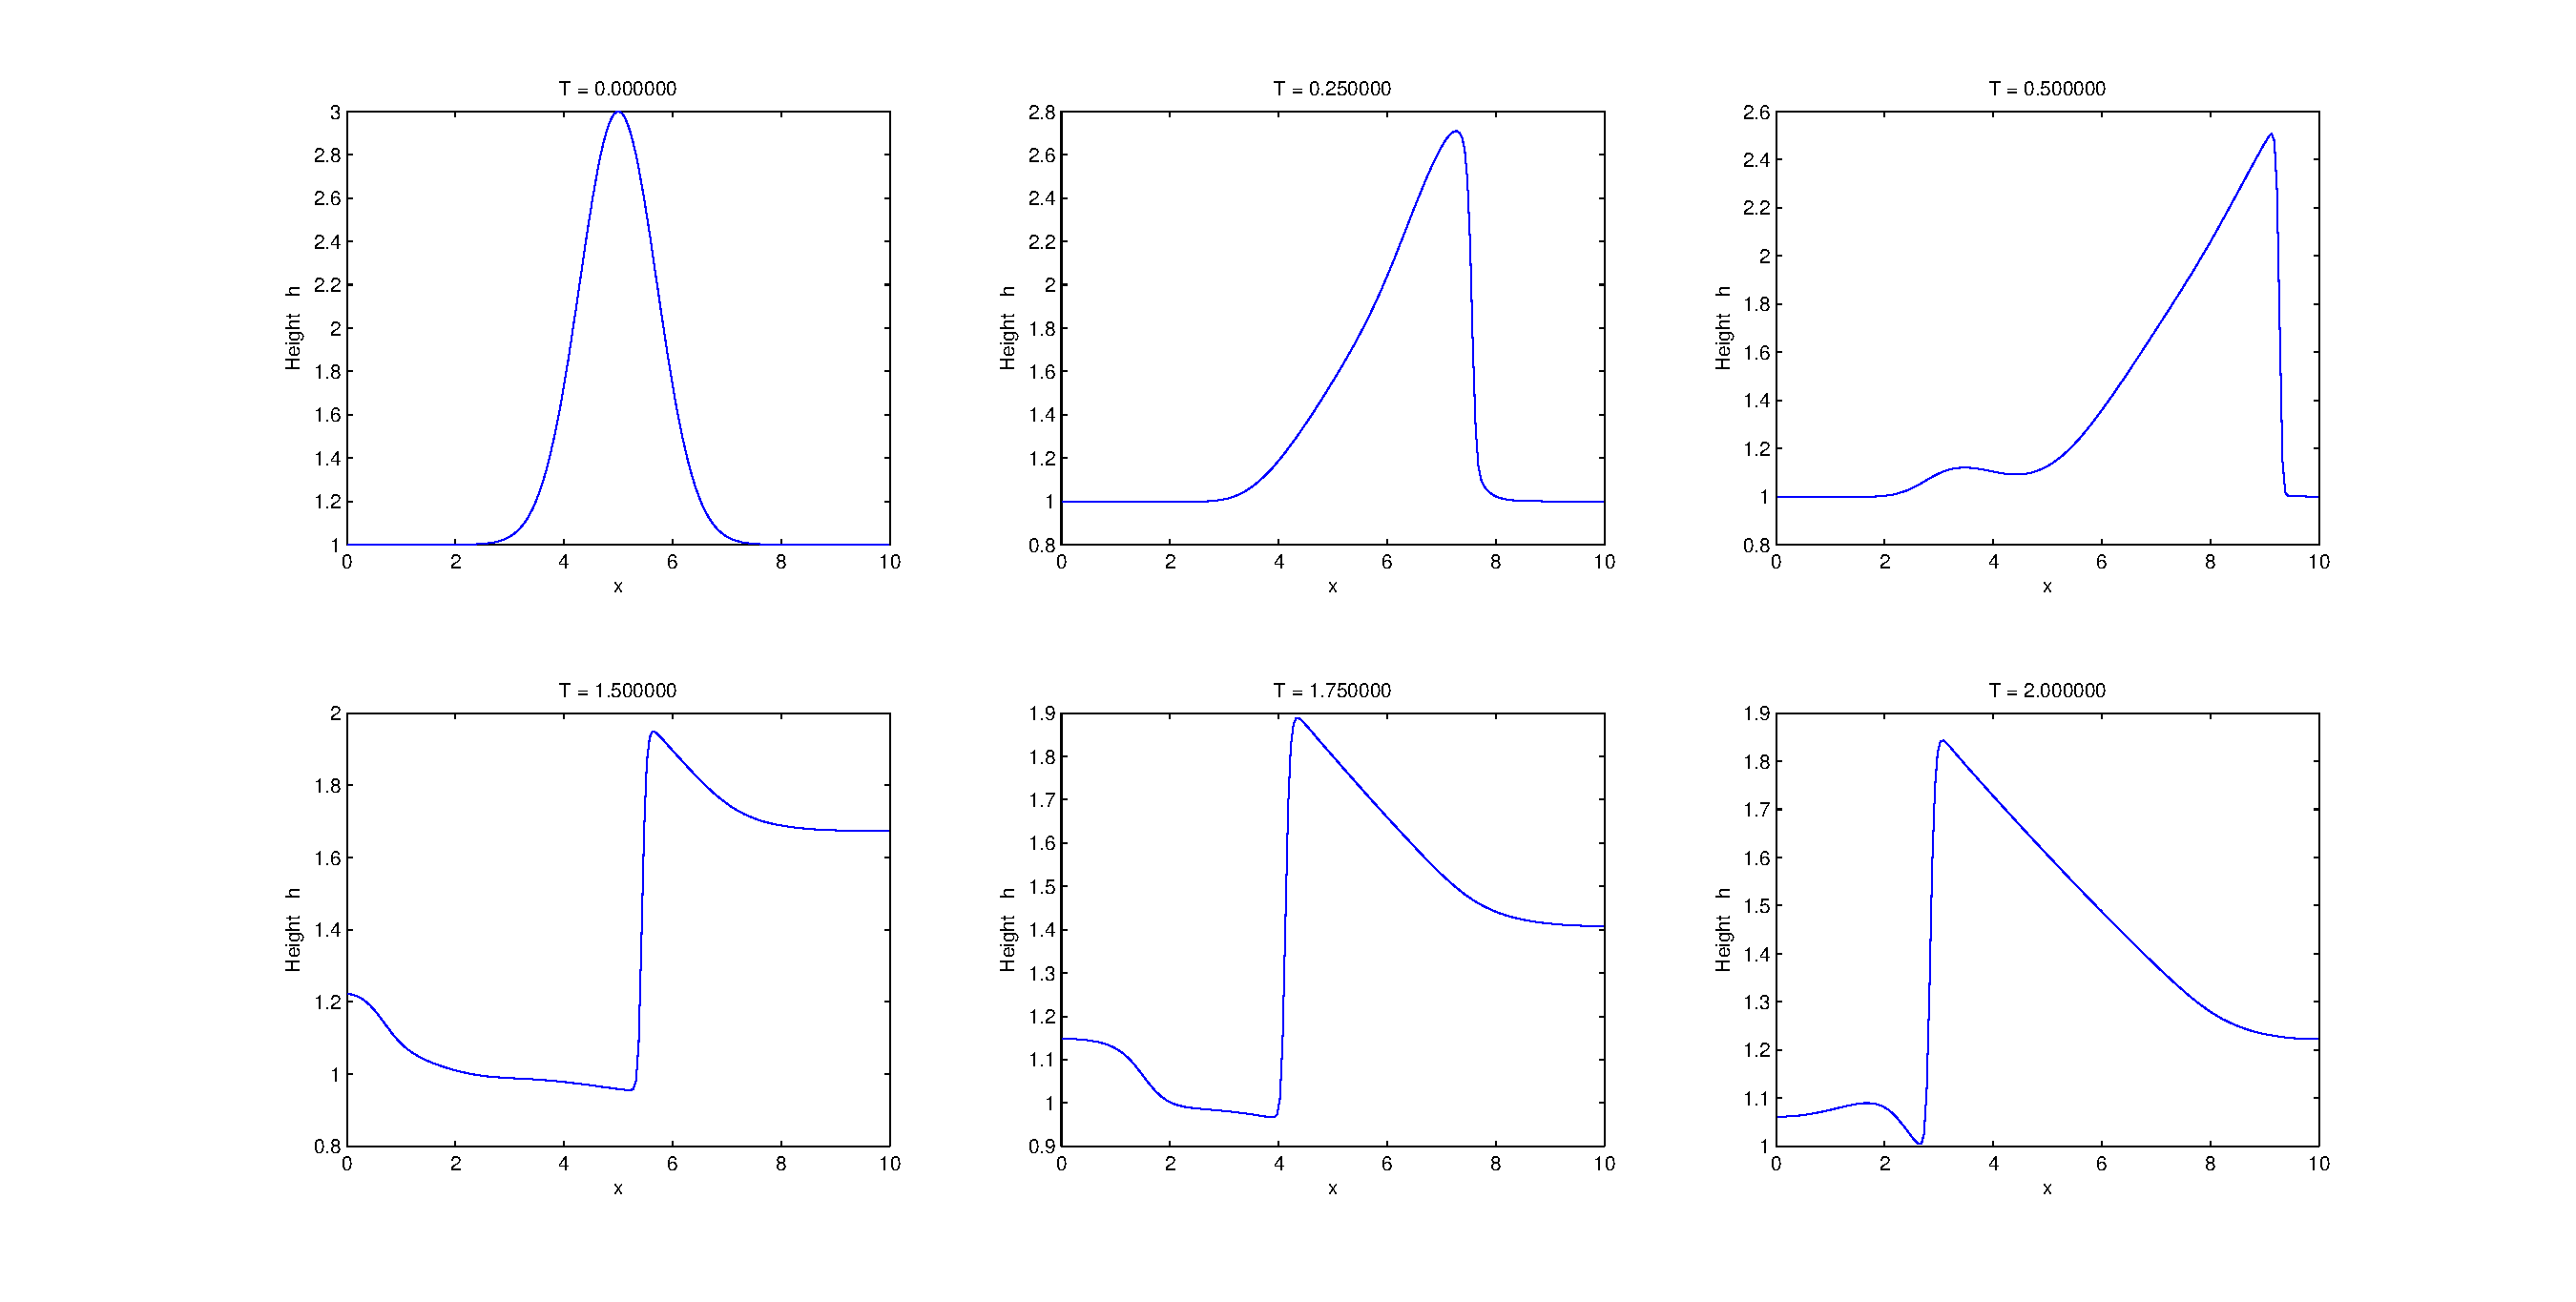
\includegraphics[scale=0.35]{higher.eps}
\caption{Results with a higher pulse $a=2H$}
\label{higher}
\end{center}
\end{figure}

Results are shown in figure \ref{higher}. We can first note that there is a lot more dissipation for this higher pulse. Indeed, for $a=H/5$, the wave had approximately the same maximum height ($1.2H$) until the end ($T_{end} = 2.5$) whereas here the wave looses more than a third of its height after 2 seconds.

We can also note that the initial data trying to produce a single pulse is not working as well as for the lower pulse. Here, we can clearly see a second wave starting to go in the left direction then bouncing back the left wall.

